\documentclass[runningheads]{llncs}
\usepackage{amssymb}
\usepackage{tikz}
\usepackage{amsmath}
\usepackage{xcolor}

\begin{document}

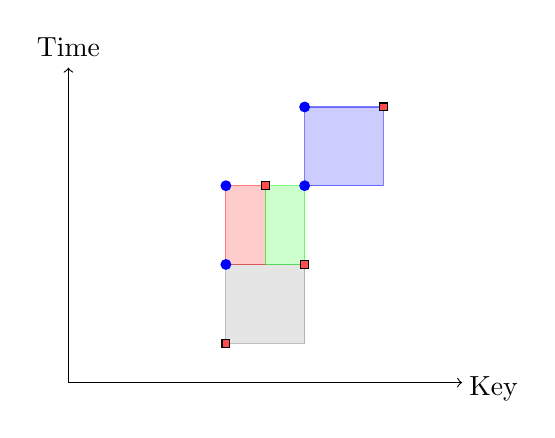
\begin{tikzpicture}[scale=.5]

\draw[->][black] (0,0) -- (10,0);
\draw[->][black] (0,0) -- (0,8);
\filldraw[gray!40!white,opacity=.5,draw=gray] (4,1) rectangle (6,3);
\filldraw[red!40!white,opacity=.5,draw=red] (5,5) rectangle (4,3);
\filldraw[green!40!white,opacity=.5,draw=green] (5,5) rectangle (6,3);
\filldraw[blue!40!white,opacity=.5,draw=blue] (8,7) rectangle (6,5);
\filldraw[draw=black,fill=red!70!white] (3.9,0.9) rectangle (4.1,1.1) (5.9,2.9) rectangle (6.1,3.1) (4.9,4.9) rectangle (5.1,5.1) (7.9,6.9) rectangle (8.1,7.1)   ;

\filldraw[blue] (4,3) circle (3.5pt) (4,5) circle (3.5pt) (6,5) circle (3.5pt) (6,7) circle (3.5pt);

\draw[black](10.8,0.4)node[anchor=north]{Key} (0,9)node[anchor=north]{Time};
\end{tikzpicture}

\end{document}